\chapter{Requisitos do Sistema}

\section{Análise e Levantamento dos Requisitos}
\subsection{Criação do grupo com os elementos da casa/apartamento}
A aplicação a desenvolver deverá suportar o registo das despesas e a gestão do seu pagamento por parte de moradores registados. Para tal é necessário que cada morador efetue um regiso fornecendo o seu nome, e-mail, número de telemóvel e data de nascimento.

O utilizador que convidar os restantes será considerado adminstrador do sistema. 

Após o registo será associada uma conta corrente, esta que permitirá a gestão do saldo (estão incluidas dividas) de cada morador. 


\subsection{Gestão das contas}
 O morador deverá efetuar um pagamento, que será creditado na conta corrente do morador. 
 
 O pagamento pode ser efetuado com valores relativamente grandes ao qual é debitado consoante é necessário ou depósitos da quantia necessária para pagar a/s despesa/s em causa. 
 
 Existirá um saldo global da casa, este que é o somatório de todas as contas correntes dos moradores, este saldo é administrado por um Adminstrador. 
 
 Existem dois tipos de despesas distintos: a despesa recorrente referente a despesas mensais como a água, luz, renda, etc; 
 a despesa extra referente a por exemplo arranjos de material na casa. 
 
 Cada morador deverá pagar uma fração relativa à despesa. 
 
 Cada despesa a pagar tem a si associado um tipo. 
 
 

\section{Base de dados }
A aplicação necessitará de uma implementação de uma base de dados para gerir os elementos que pertencem ao grupo assim como as despesas efetuadas pelos moradores. 

\chapter{Arquitetura da Aplicação}

\section{Modelo de Dominio }
Todo e qualquer projeto possui um domínio específico. O modelo de domínio deve capturar os seguintes pontos: as entidades, os relacionamentos entre as entidades e o vocabulário de domínio do problema. Para além disso também deve ser uma visão estática do problema onde é possível representar as regras de negócio invariantes no tempo. Ou seja, o modelo de domínio é a base para a análise de requisitos.

No que diz respeito à aplicação, como é dito na introdução, queremos desenvolver uma aplicação capaz de suportar o registo das despesas e a gestão do seu pagamento por parte dos moradores registados.


\begin{figure}[htb!]
	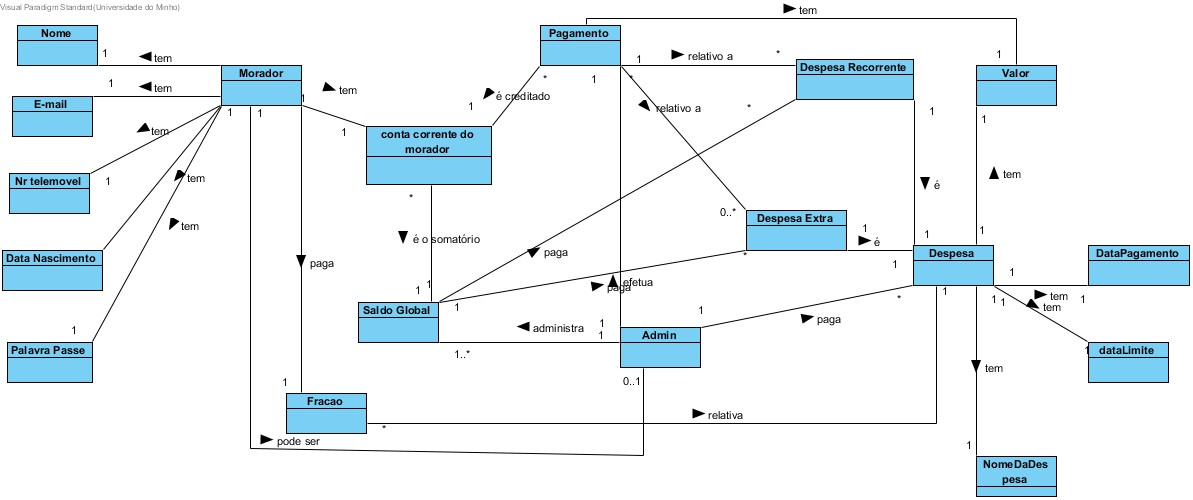
\includegraphics[scale=0.566]{ModeloDominio}  
	\caption{Modelo Dominio}  
\end{figure}

O morador necessita de fornecer o nome, e-mail, número de telemovel e data de nascimento, para efetuar o login. 

Como se pode observar na figura o morador efetua pagamento relativo a despesa recorrente ou extra, assim como paga uma fração da despesa, essa fração é relativa a um tipo de despesa. 


O administrador administra o saldo global da casa/apartamento. 


\newpage

\section{Modelo de Use Case}
A segunda parte da análise de requisitos corresponde à definição dos use cases, com o objetivo de os aplicar nesta primeira fase deste trabalho prático. Nos use cases, queremos primeiramente, identificar os atores, que serão quem interagirá com o sistema.
Posterior à identificação dos atores, passamos então à identificação dos use cases, isto é, o que se pretende do sistema. No último ponto da visão orientada aos use cases, procedemos à identificação das classes de suporte à realização dos mesmo, que corresponde à especificação da funcionalidade a ser implementada.
Neste sentido, quando definimos um use case, para além de ser uma espécie de documentação, temos de ter em conta que se trata de uma unidade coerente de funcionalidade, um serviço. Define também um comportamento do sistema, sem revelar a estrutura interna, divulgando desta forma, a comunicação entre os atores e o sistema.
O conjunto de todos os use cases acaba por definir pela íntegra, toda a funcionalidade do sistema que decorre na sua essência, do diálogo entre o sistema e os atores, e a responsabilidade de resposta funcional do sistema.

\subsection{Diagrama de Use Case}


\begin{figure}[htb!]
	\centering
	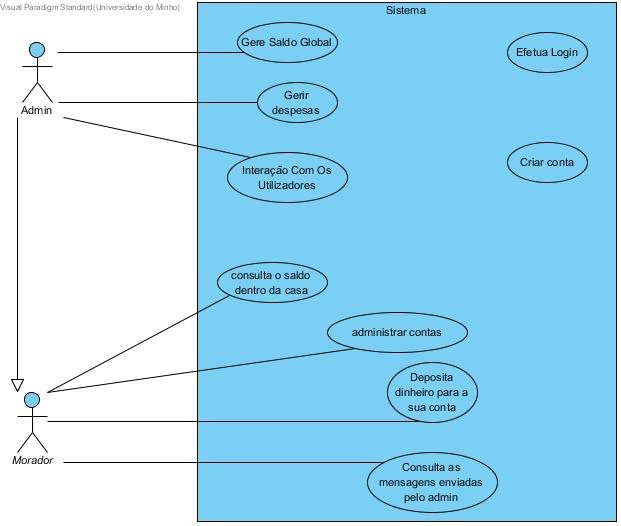
\includegraphics[scale=0.5]{UseCase}  
	\caption{Modelo Use Case}  
\end{figure}

\subsection{Subdiagramas}

\begin{figure}[htb!]
	\centering
	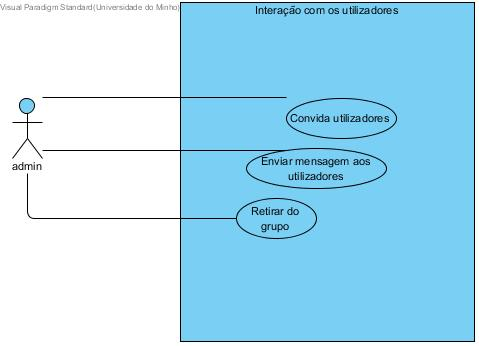
\includegraphics[scale=0.5]{InteracaoComOsUtilizadores}  
	\caption{Sub-Diagrama Interação com os Utilizadores }  
\end{figure}


\begin{figure}[htb!]
	\centering
	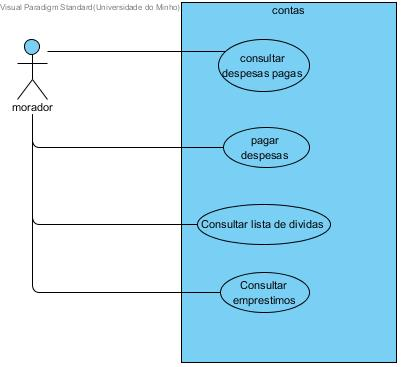
\includegraphics[scale=0.5]{despesasMorador}  
	\caption{Sub-Diagrama Despesas }  
\end{figure}


\begin{figure}[htb!]
	\centering
	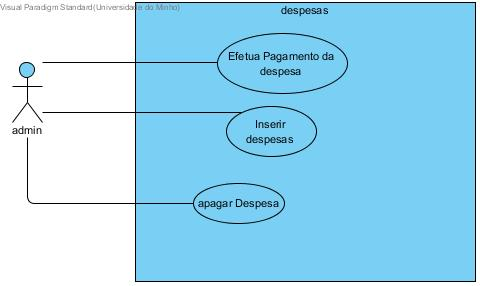
\includegraphics[scale=0.5]{GerirDespesas}  
	\caption{Sub-Diagrama gerir despesa }  
\end{figure}

\newpage
\section{Mockups}

\begin{figure}[htb!]
	\centering
	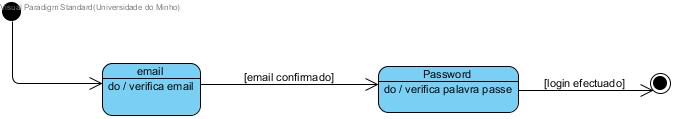
\includegraphics[scale=0.4]{Login}  
	\caption{Login}  
\end{figure}

\begin{figure}[htb!]
	\centering
	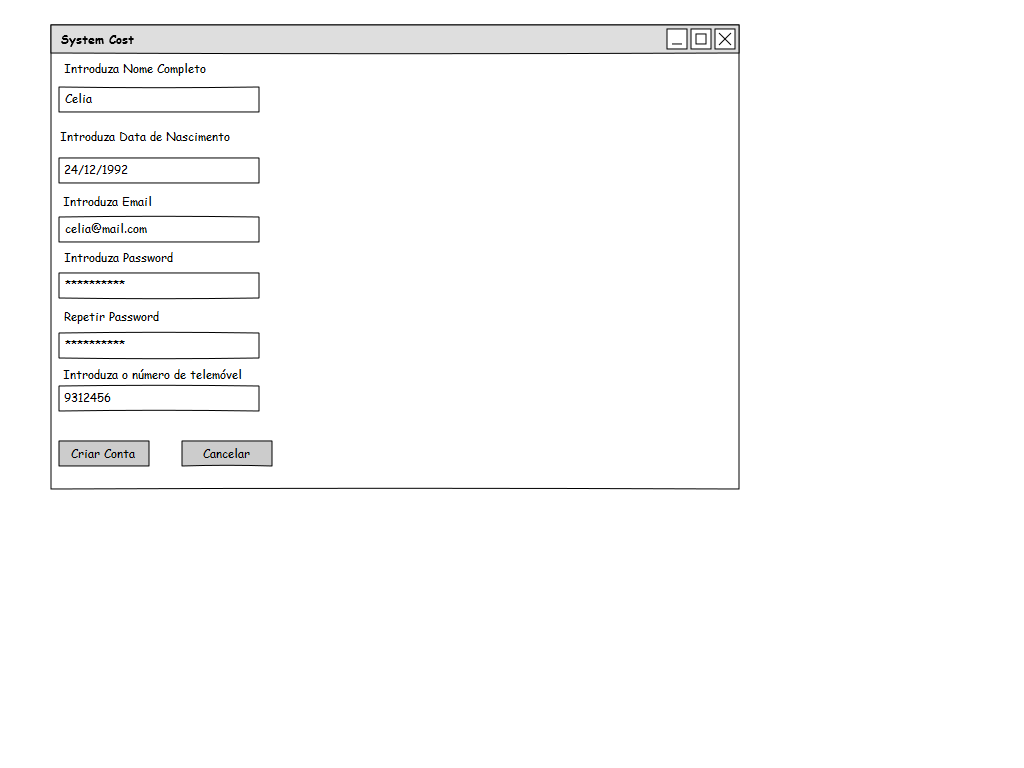
\includegraphics[scale=0.4]{CriarConta}  
	\caption{Criar nova Conta }  
\end{figure}

\begin{figure}[htb!]
	\centering
	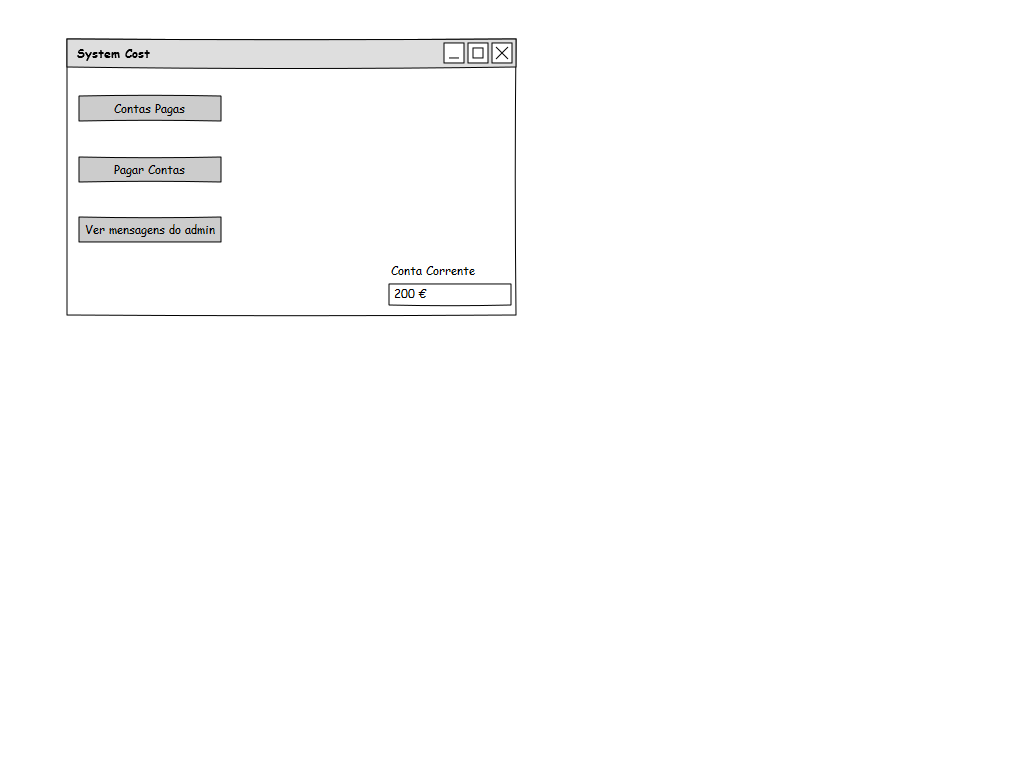
\includegraphics[scale=0.4]{UtilizadorNormal}  
	\caption{Utilizador Normal }  
\end{figure}

\begin{figure}[htb!]
	\centering
	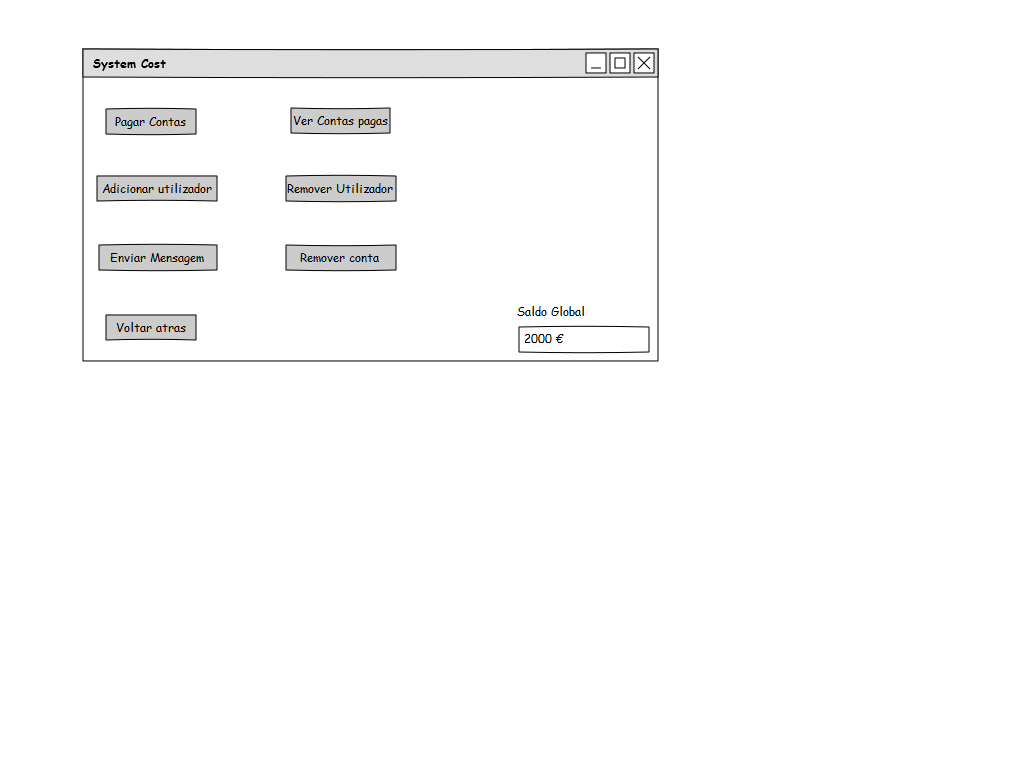
\includegraphics[scale=0.4]{Admin}  
	\caption{Privilégios de administrador }  
\end{figure}




